\documentclass[mat1]{fmfdelo}
\usepackage{graphicx}
\usepackage{amsmath}
\usepackage[shortlabels]{enumitem}
% \documentclass[fin1]{fmfdelo}
% \documentclass[isrm1]{fmfdelo}
% \documentclass[mat2]{fmfdelo}
% \documentclass[fin2]{fmfdelo}
% \documentclass[isrm2]{fmfdelo}

% naslednje ukaze ustrezno napolnite
\avtor{Matej Novoselec}

\naslov{Schwarzov princip zrcaljenja za harmonične funkcije}
\title{Schwarz Reflection Principle for Harmonic Functions}

% navedite ime mentorja s polnim nazivom: doc.~dr.~Ime Priimek,
% izr.~prof.~dr.~Ime Priimek, prof.~dr.~Ime Priimek
% uporabite le tisti ukaz/ukaze, ki je/so za vas ustrezni
\mentor{prof. dr. Barbara Drinovec Drnovšek}
% \mentorica{}
% \somentor{}
% \somentorica{}
% \mentorja{}{}
% \mentorici{}{}

\letnica{2023} % leto diplome

%  V povzetku na kratko opišite vsebinske rezultate dela. Sem ne sodi razlaga organizacije dela --
%  v katerem poglavju/razdelku je kaj, pač pa le opis vsebine.
\povzetek{}

%  Prevod slovenskega povzetka v angleščino.
\abstract{}

% navedite vsaj eno klasifikacijsko oznako --
% dostopne so na www.ams.org/mathscinet/msc/msc2020.html
\klasifikacija{}
\kljucnebesede{} % navedite nekaj ključnih pojmov, ki nastopajo v delu
\keywords{} % angleški prevod ključnih besed

\zapisiMetaPodatke  % poskrbi za metapodatke in veljaven PDF/A-1b standard

% aktivirajte pakete, ki jih potrebujete
% \usepackage{tikz}

% za številske množice uporabite naslednje simbole
\newcommand{\R}{\mathbb R}
\newcommand{\N}{\mathbb N}
\newcommand{\Z}{\mathbb Z}
\newcommand{\C}{\mathbb C}
\newcommand{\Q}{\mathbb Q}

% matematične operatorje deklarirajte kot take, da jih bo Latex pravilno stavil
% \DeclareMathOperator{\conv}{conv}

% vstavite svoje definicije ...
%  \newcommand{}{}

\begin{document}

\section{Uvod}
V diplomski nalogi bomo spoznali osnovne lastnosti harmoničnih fukcij, ki jih bomo proti koncu s pridom uporabili za dokaz glavnega izreka, katerega ime nosi naslov naloge.
Vlekli bomo številne vzporednice s kompleksno analizo, gre namreč za področje, močno povezano s študijo holomorfnih funkcij.

V prvem poglavju bomo spoznali, kaj so harmonične funkcije in poudarili, katere njihove lastnosti bodo za nadaljevanje pomembne. Ogledali si bomo tudi njihov odnos s holomorfnimi funkcijami. 
V drugem poglavju bomo spoznali Dirichletov problem za enotski disk, ki nam bo dal osnovo za definicijo Poissonovega jedra in Poissonovega integrala. Ogledali si bomo nekaj lastnosti obeh definiranih pojmov in z njuno pomočjo rešili Dirichletov problem za enotski disk.
Tretje poglavje je namenjeno karakterizaciji harmoničnih funkcij s pomočjo lastnosti povprečne vrednosti in analizi pomembnosti te karakterizacije. 
V zadnjem poglavju bomo s pomočjo orodij, spoznanih v prejšnih poglavjih, navedli in dokazali glavni izrek diplomskega dela - Schwarzov princip zrcaljenja za harmonične funkcije.
%\section*{Slovar strokovnih izrazov}
%
%\geslo{}{}
%\geslo{}{}

%------------------------------------------------------------
\newpage
\section{Harmonične funkcije}
    \begin{definicija}
        \label{harm}
        Naj bo $U$ odprta podmnožica v $\mathbb{R}^n$. Naj bo $u$ funkcija, definirana na $U$ in naj bo na definicijskem območju dvakrat zvezno odvedljiva.  
        Pravimo, da je funkcija $u(x_1, x_2, \dots, x_n)$ \emph{harmonična}, če velja
        $$
        \frac{\partial^2 u}{\partial x_1 ^ 2} +  \frac{\partial^2 u}{\partial x_2 ^ 2} + \dots + \frac{\partial^2 u}{\partial x_n ^ 2} = 0.
        $$
        Operatorju $\Delta  = \frac{\partial^2}{\partial x_1 ^ 2} +  \frac{\partial^2}{\partial x_2 ^ 2} + \dots + \frac{\partial^2}{\partial x_n ^ 2}$ pravimo \emph{Laplaceov operator} in pišemo
        $$
        \Delta u = 0.
        $$
    \end{definicija}

    Pogoj za harmoničnost podaja Laplaceovo parcialno diferencialno enačbo, zapisano bodisi s Laplaceovim operatorjem ali razpisano s parcialnimi odvodi drugega reda. 
    Funkcija je torej harmonična, če zadošča zgoraj zapisani parcialni diferencialni enačbi. 
    %Po tihem tu seveda privzemamo obstoj (vsaj) drugih parcialnih odvodov, saj drugače o harmoničnosti funkcije ne moremo govoriti.

    \begin{opomba}
        Vredno je omeniti, da v zgornji definiciji nismo specificirali, ali gre pri funkciji $u$ za realno ali kompleksno funkcijo. 
        Pojem harmoničnosti smo definirali v splošnem, torej tako za kompleksne kot tudi realne funkcije.
        Znotraj diplomske naloge se bomo omejili na funkcije dveh realnih spremenljivk ali funkcijo ene kompleksne spremenljivke, ki jo bomo nato delili na realni in imaginarni del ($z = x + iy $) in na ta način prešli nazaj na funkcije dveh realnih spremenljivk.
        \newline
        Pogoj za harmoničnost takrat zapišemo kot: 
            $$
                \Delta u = \frac{\partial^2 u}{\partial x ^ 2} +  \frac{\partial^2 u}{\partial y ^ 2}= 0.
            $$
    \end{opomba}

    \begin{definicija}
        \emph{Območje} $D$ je povezana odprta množica v $\mathbb{R}^n$.
        Če obstaja $a \in D$, da za vse $b \in D$ in vse $t \in [0,~1]$ tudi $t a + (1-t)b \in D$, pravimo, da je $D$ \emph{zvezdasto območje}.
    \end{definicija}


    \begin{trditev}
        \label{hh}
        Naj bo $U \subseteq \mathbb{C}$ odprta množica. Naj bo $f = u + iv$ holomorfna funkcija, $u$ in $v$ pa realni funkciji, definirani na $U$. Potem sta realni funkciji $u$ in $v$ harmonični na $U$.
    \end{trditev}

    \begin{dokaz}
        Ker je $f$ holomorfna, zadošča Cauchy-Riemannovemu sistemu enačb prek katerih lahko bralec sam hitro preveri, da trditev drži. Dokaz je natančneje naveden v \cite{osnova}, na strani $55$.
    \end{dokaz}

    \begin{opomba}
        Če označimo $u = \text{Re}{f}$ in $v = \text{Im}{f}$, nam zgornja trditev v resnici pove, da sta realni in imaginarni del holomorfne funkcije harmonični funkciji. 
    \end{opomba}

    \begin{definicija}
        Naj bo $u$ realna harmonična funkcija, definirana na območju $D$. Če obstaja realna harmonična funkcija $v$, definirana na $D$, da je funkcija $f = u + iv$ na $D$ holomorfna, potem funkciji $v$ pravimo \emph{harmonična konjugiranka funkcije $u$ na $D$}.    
    \end{definicija}

    \begin{trditev}
        \label{konj}
        Naj bo $u$ realna harmonična funkcija, definirana na zvezdastem območju $D$. Potem za $u$ na $D$ obstaja harmonična konjugiranka $v$ in je do konstante natančno enolično določena. 
    \end{trditev}
    \begin{dokaz}
        Konstrukcijo harmonične konjugiranke, si bralec za primer, ko je zvezdasto območje kar odprt disk lahko ogleda v \cite{osnova}, na strani $56$ in $57$. 
        Ideja dokaza za splošno zvezdasto območje je podobna. 
    \end{dokaz}

    \begin{opomba}
        V duhu zgornjih dveh trditev, je velikokrat smiselno na realno harmonično funkcijo $u$ gledati kot na realni del holomorfne funkcije $f = u + iv$, kjer je $v$ njena harmonična konjugiranka. To že nakazuje, da se bodo nekatere lepe lastnosti holomorfnih funkcij prenesle tudi na harmonične funkcije.
    \end{opomba}
    %%V duhu zgornjih dveh opomb, opazimo, da lahko kompleksno funkcijo $f$, zapišemo v obliki realnega in imaginarnega dela oziroma kot $f = u + i v$, s pomočjo nekih realnih funkcij (dveh spremenljivk) $u$ in $v$, ter lahko zaradi linearnosti parcialnih odvodov sklepamo, da je za harmoničnost $f$ kot kompleksne funkcije, dovolj zahtevati harmoničnost $u$ in $v$ kot realnih funkcij.
    %%Podoben argument nam da vedeti, da nam harmoničnost $f = u + iv$, implicira tudi harmoničnost $u$ in $v$. 
    \begin{opomba}
        \label{lin}
        Zaradi linearnosti parcialnih odvodov, je tudi linearna kombinacija harmoničnih funkcij harmonična. To bomo pri reševanju enega izmed glavnih problemov diplomskega dela s pridom uporabili.
    \end{opomba}
    \begin{opomba}
        V literaturi se v definiciji harmoničnosti za funkcijo $u$ pojavlja tudi zahteva, da je funkcija gladka, oziroma $u \in C^{\infty}$. V zgornji definiciji zahtevamo le obstoj drugih parcialnih odvodov, oziroma $u \in C^2$. 
        Da sta definiciji med seboj ekvivalentni, potrdi spodnja trditev. 
    \end{opomba}
    \begin{trditev}
        \label{gladkosth}
        Naj bo $u$ realna harmonična funkcija definirana na območju $D$. Potem je $u$ na $D$ gladka, oziroma $u \in C^{\infty}(D)$. 
    \end{trditev}
    \begin{dokaz}
        Ker je  $D$ odprta množica, lahko za vsako točko $z \in D$ najdemo dovolj majhno zvezdasto okolico $U_z$, da bo okolica v celoti vsebova v $D$. Dovolj je vzeti kar dovolj majhen disk. 
        Po trditvi \ref{konj} na $U_z$ obstaja harmonična konjugiranka $v$, da je $f = u+ iv$ na $U_z$ holomorfna, ter zato na $U_z$ tudi gladka. Sledi, da je na $U_z$ gladka tudi funkcija $u$.
        Ker smo za vsako točko iz $D$ našli odprto okolico na kateri je funkcija $u$ gladka, je $u$ gladka na celotnem definicijskem območju.
    \end{dokaz}

\section{Lastnost povprečne vrednosti}

    \begin{definicija}  
        Naj bo $h$ zvezna funkcija, definirana na območju $D$. Denimo, da za $z_0 \in D$ in $r > 0$ velja $\overline{\mathbb{D}}(z_0, r) \subseteq D$. \emph{Povprečje funkcije} $h$ na $\overline{\mathbb{D}}(z_0, r)$ definiramo kot:
        $$
            A(r) = \int_{0}^{2 \pi}{h \big(z_0 + r e^{i\theta}\big)\frac{d\theta}{2 \pi}}.
        $$
    \end{definicija}
    \begin{trditev}
        \label{zvpov}
        Naj bo $h$ zvezna funkcija, definirana na območju $D$, ter denimo, da za $z_0 \in D$ in $r > 0$ velja $\overline{\mathbb{D}}(z_0, r) \subseteq D$. 
        Potem je $A(r)$ zvezna na $(0,~r]$ in velja: $\lim_{r \to 0}{A(r)} = h(z_0)$.
    \end{trditev}
    \begin{dokaz}
        Ker je povprečje zvezne funkcije definirano kot integral zvezne funkcije, je funkcija $A(r)$ zvezna na $(0,~r]$. Drugi del trditve dokažimo po definiciji.
        Naj bo $\epsilon > 0$ poljubno majhen. Velja:
        $$
            |A(r) - h(z_0)| = \bigg|\int_{0}^{2\pi} \big[h(z_0 + r e^{i\theta})  - h(z_0)\big] \frac{d\theta}{2\pi} \bigg| \leq \int_{0}^{2 \pi} \big| h(z_0 + r e^{i\theta}) - h(z_0) \big| \frac{d\theta}{2 \pi}.
        $$
        Ker je $h$ zvezna, obstaja $\delta > 0$, da za vsak $|r| < \delta$ in vsak $\theta \in [0,~2\pi]$ velja \mbox{$|h(z_0 + r e^{i\theta}) - h(z_0)| < \epsilon$}.
        Za vsak $r$, ki je manjši od $\delta$ torej $|A(r) - h(z_0)| < \epsilon$. Ker je bil $\epsilon$ poljubno majhen, res velja $\lim_{r \to 0}{A(r)} = h(z_0)$.
    \end{dokaz}

    \begin{definicija}
        Naj bo $h$ zvezna funkcija, definirana na območju $D \subseteq \C$. Pravimo, da ima funkcija $h$ na $D$ \emph{lastnost povprečne vrednosti}, če za vsak $z_0 \in D$ obstaja $\epsilon_0 > 0$, da je $\overline{\mathbb{D}}(z_0, \epsilon_0) \subseteq D$ in za vsak $0 < \epsilon \leq \epsilon_0 $ velja:
        $$
            h(z_0) = \frac{1}{2 \pi} \int_{0}^{2 \pi}{h(z_0 + \epsilon e^{i \theta}) d\theta}.
        $$
    \end{definicija}
    \begin{opomba}
        Definicija nam pove, da ima zvezna funkcija $h$ na območju $D \subseteq \C$ lastnost povprečne vrednosti, če za vsak $z_0$ iz $D$ velja, 
        da je $h(z_0)$ povprečje vrednosti $h(z)$, kjer $z$ teče po majhni krožnici s središčem v $z_0$.
    \end{opomba}
    \begin{trditev}
        \label{linlpv}
        Linearna kombinacija funkcij z lastnostjo povprečne vrednosti je funkcija z lastnostjo povprečne vrednosti. 
    \end{trditev}
    \begin{dokaz}
        Trditev sledi iz linearnosti integrala.
    \end{dokaz}

    %\begin{lema}
    %    \label{lema_princip_max}
    %    Naj bo $u$ zvezna realna funkcija, definirana na območju $D$. Naj ima $u$ na $D$ lastnost povprečne vrednosti in naj obstaja $M \in \mathbb{R}$, da za vsak $z \in D$ velja: $u(z) \leq M$. 
    %    Če obstaja $z_0 \in D$, da velja: $u(z_0) = M$, potem je $u(z) = M$ za vsak $z \in D$.
    %\end{lema}
    %\begin{dokaz}
    %    Ker je $u$ na $D$ zvezna, je množica $A = \{z \in D~|~u(z) < M\}$ odprta. Po definiciji dokažimo, da je odprta tudi množica $B = \{z \in D~|~u(z) = M\}$. Naj bo $z_1 \in B$. Ker je $D$ odprta, obstaja $\rho_{z_1}$, da je za vsak $0 < r < \rho_{z_1}$ tudi $\overline{\mathbb{D}}(z_1, r) \subseteq D$. 
    %    Funkcija $u$ ima na $D$ lastnost povprečne vrednosti, zato velja:
    %    $$
    %        u(z_1) = \int_{0}^{2\pi}{u(z_1 + re^{i\theta}) \frac{d\theta}{2\pi}},~\text{za vsak}~0<r<\rho_{z_1}, 
    %    $$
    %    oziroma: 
    %    $$
    %    0 = \int_{0}^{2\pi}{\left[u(z_1) - u(z_1 + re^{i\theta}) \right]\frac{d\theta}{2\pi}},~\text{za vsak}~0<r<\rho_{z_1}.
    %    $$
    %    Ker je integrand nenegativen in zvezen, integral pa enak nič, je integrand enak nič. 
    %    Sledi, da je $M = u(z_1) = u(z_1 + r e^{i \theta})$, za vsak $\theta \in [0,~2\pi]$ in vsak $0 < r < \rho_{z_1}$, oziroma ima poljuben $z_1 \in B$ okolico, ki je vsebovana v $B$. Torej je $B$ odprta.
    %    Predpostavka nam pove, da za vsak $z \in D$ velja $u(z) \leq M$, zato je $D$ disjunktna unija množic $A$ in $B$. Ker je $D$ povezana, $A$ in $B$ pa odprti množici, je ena izmed niju prazna, druga pa posledično enaka $D$. Ker po predpostavki $B$ vsebuje $z_0$, je $A$ prazna, $B$ pa je enaka $D$. Sledi, da je $u(z) = M$ za vsak $z \in D$. 
    %\end{dokaz}

    \begin{trditev}[Princip maksima za funkcije z lastnostjo povprečne vrednosti]
        \label{pm_lpv}
        Naj bo $h$ zvezna kompleksna funkcija, definirana na območju $D$. Naj ima $h$ na $D$ lastnost povprečne vrednosti in naj obstaja $M \in \mathbb{R}$, da velja $|h(z)| \leq M$ za vsak $z \in D$. 
        Če obstaja $z_0 \in D$, da je $|h(z_0)| = M$, potem je funkcija $h(z)$ na $D$ konstantna. 
    \end{trditev}
    \begin{dokaz}
        Ker je $|h(z_0)| = M$, obstaja $\varphi \in [0,~2\pi]$, da velja: \mbox{$h(z_0) = M e^{i \varphi}$}.
        Definirajmo: $H(z) = h(z) e^{-i\varphi},~z \in D$. Po trditvi \ref{linlpv} ima $H$ na $D$ lastnost povprečne vrednosti. Opazimo, da velja: $|H(z)|  \leq M$ za vsak $z \in D$, obenem pa \mbox{$H(z_0) = M$}.
        Ker je funkcija $H$ na $D$ zvezna, $\{H(z_0)\}$ pa zaprta množica, je njena praslika \mbox{$A = \{z \in D~|~H(z) = H(z_0) = M\}$} prav tako zaprta množica. Po definiciji dokažimo, da je $A$ tudi odprta množica. 
        Naj bo $z_1 \in A$. Ker je $D$ odprta, obstaja $\rho_{z_1}$, da je za vsak $0 < r < \rho_{z_1}$ tudi $\overline{\mathbb{D}}(z_1, r) \subseteq D$. 
        Funkcija $H$ ima na $D$ lastnost povprečne vrednosti, zato velja:
        $$
            H(z_1) = \int_{0}^{2\pi}{H(z_1 + re^{i\theta}) \frac{d\theta}{2\pi}},~\text{za vsak}~0<r<\rho_{z_1}.
        $$
        Ker je $z_1 \in A$, velja $H(z_1) = M$, ter zato $\text{Re}[H(z_1)] = H(z_1)$. 
        Sledi:
        $$
        H(z_1) = \text{Re}[H(z_1)] = \int_{0}^{2\pi}{\text{Re}[H(z_1 + re^{i\theta})]~\frac{d\theta}{2\pi}},~\text{za vsak}~0<r<\rho_{z_1},
        $$
        oziroma:
        $$
        0 = \int_{0}^{2\pi}{\left(H(z_1) - \text{Re}[H(z_1 + re^{i\theta})] \right)\frac{d\theta}{2\pi}},~\text{za vsak}~0<r<\rho_{z_1}.
        $$
        Vemo, da za vsak $z \in D$ velja: $|H(z)| \leq M = H(z_1)$, zato za vsak $z \in D$ velja: $\text{Re}[H(z)] \leq |H(z)| \leq H(z_1)$.
        Sedaj vemo, da je integrand integrala nenegativen in zvezen, integral pa enak nič, zato je integrand enak nič. 
        Sledi, da je \mbox{$H(z_1) = \text{Re}[H(z_1 + r e^{i \theta})]$}, za vsak $\theta \in [0,~2\pi]$ in vsak $0 < r < \rho_{z_1}$. Definicija absolutne vrednosti nam da: $|H(z)| = \sqrt{\text{Re}[H(z)]^2 + \text{Im}[H(z)]^2}$. 
        Ker vemo, da za vsak $z \in D$ velja: $|H(z)| \leq H(z_1) = M$, za vsak $w \in \mathbb{D}(z_1,\rho_{z_1})$ pa $H(z_1) = \text{Re}[H(w)]$, sledi, da je za vsak $w \in \mathbb{D}(z_1,\rho_{z_1})$: $\text{Im}[H(w)] = 0$, oziroma: $H(w) = H(z_1)$. 
        Poljuben $z_1 \in A$ ima torej odprto okolico, ki je vsebovana v $A$. Torej je $A$ odprta.
        Predpostavka trditve nam pove, da $A$ ni prazna, saj $z_0 \in A$. Ker je $D$ povezana, $A$ pa odprta in hkrati zaprta neprazna množica, velja $A = D$. 
        Po definiciji množice $A$ je zato funkcija $H(z)$ na $D$ konstantna. \mbox{Posledično je na $D$ konstantna tudi funkcija $h(z)$.} 
    \end{dokaz}

    \begin{posledica}
        \label{posledica_pm_lpv}
        Naj bo $h$  kompleksna funkcija, definirana na omejenem območju $D$. Naj bo $h$ zvezna na $\overline{D}$ in naj ima na $D$ lastnost povprečne vrednosti. 
        Če obstaja $M \in \mathbb{R}$, da velja $|h(z)| \leq M$ za vsak $z \in \partial D$, potem velja $|h(z)| \leq M$ za vsak $z \in \overline{D}$. 
    \end{posledica}
    \begin{dokaz}
        Ker je funkcija $h$ zvezna na kompaktnem območju $\overline{D}$, na $\overline{D}$ zavzame minimum in maksimum. Posledično funkcija $|h|$ na $\overline{D}$ zavzame maksimum. 
        Torej $|h|$ zavzame maksimum na $D$ ali na $\partial D$. Če funkcija $|h|$ maksimum zavzame na $D$, potem je po trditvi \ref{pm_lpv} funkcija $h$ na $D$ konstantna. Ker je $h$ zvezna na $\overline{D}$, je $h$ konstantna celo na $\overline{D}$. 
        Sledi, da $h$ maksimum gotove zavzame na $\partial D$ iz česar lahko sklepamo želeno.
    \end{dokaz}

    \begin{trditev}
        Naj bo $f$ holomorfna funkcija na območju $D$. Potem ima funkcija $f$ na $D$ lastnost povprečne vrednosti.
    \end{trditev}
    \begin{dokaz}
        Ker je funkcija $f$ na območju $D$ holomorfna, lahko uporabimo Cauchyjevo integralsko formulo za vsak zaprt disk, ki je v celoti vsebovan v $D$. Za vsak $z \in D$ in vsak $r > 0$, kjer je $\overline{\mathbb{D}}(z,r) \subseteq \mathbb{D}$ torej velja:
        $$
        f(z) = \frac{1}{2 \pi i} \int_{\partial \overline{\mathbb{D}}(z, r)}{\frac{f(\xi)}{\xi  - z}}d\xi.
        $$
        Ko rob diska parametriziramo z $\xi = z + r e^{i \varphi}$, dobimo:
        $$
        f(z) = \frac{1}{2 \pi} \int_{0}^{2\pi}{f(z + re^{i\varphi})}d\varphi.
        $$
    \end{dokaz}

    \begin{trditev}
        \label{harmonicnapovp}
        Naj bo $u$ harmonična funkcija, definirana na območju $D \subseteq \C$. Naj bo $z_0 \in D$ in $\rho > 0$, da velja $\overline{\mathbb{D}}(z_0, \rho) \subseteq D$. Za vsak $0 < r < \rho$ potem velja:
            $$
                u(z_0) = \frac{1}{2 \pi} \int_{0}^{2 \pi}{u(z_0 + r e^{i \theta}) d\theta}.
            $$
    \end{trditev}
    \begin{dokaz}
        Na $\overline{\mathbb{D}}(z_0, \rho) \subseteq D$ označimo $P = -\frac{\partial u}{\partial y}$ in $Q = \frac{\partial u}{\partial x}$, ter uporabimo Greenovo integralsko formulo:
        $$
            \int_{\partial \overline{\mathbb{D}}(z_0, \rho)}{P dx + Q dy} = \iint_{\overline{\mathbb{D}}(z_0, \rho)}{\bigg(\frac{\partial Q}{\partial x} - \frac{\partial P}{\partial y}\bigg)dx dy}.
        $$ 
        Sedaj upoštevajmo harmoničnost funkcije $u$ in vstavimo v Greenovo formulo:
        $$
        \int_{\partial \overline{\mathbb{D}}(z_0, \rho)}{-\frac{\partial u}{\partial y} dx + \frac{\partial u}{\partial x} dy} = \iint_{\overline{\mathbb{D}}(z_0, \rho)}{\bigg(\frac{\partial^2 u}{\partial x^2} + \frac{\partial^2 u}{\partial y^2}\bigg)dx dy} = 0. 
        $$
        Rob diska lahko pri $z_0 = x_0 + iy_0$ parametriziramo z $x(\theta) = x_0 + \rho \cos(\theta),~y(\theta) = y_0 + \rho \sin(\theta)$. Ko to vstavimo v zgornjo enakost, dobimo:
        $$
        0 = \rho \int_{0}^{2 \pi}{\bigg[\frac{\partial u}{\partial x} \cos(\theta) + \frac{\partial u}{\partial y} \sin(\theta)\bigg] d\theta} = \rho \int_{0}^{2\pi}{\frac{\partial u}{\partial \rho}\big({z_0 + \rho e^{i\theta}\big)d\theta}}.
        $$
        Ker je $u$ harmonična, je po trditvi \ref{gladkosth} gladka, zato lahko zamenjamo limitna procesa integriranja in odvajanja. Delimo z $2\pi \rho$ in zapišemo:
        $$
        0 = \frac{\partial}{\partial \rho} \int_{0}^{2\pi}{u\big({z_0 + \rho e^{i\theta}\big)\frac{d\theta}{2 \pi}}}.
        $$
        Sledi, da je vrednost zgornjega integrala konstantna, za vsak $0 <r < \rho$. Obstaja torej $c \in \mathbb{C}$, da je: 
        $$
        \int_{0}^{2\pi}{u\big({z_0 + r e^{i\theta}\big)\frac{d\theta}{2 \pi}}} = c,~\text{za vsak}~ 0 < r < \rho.
        $$
        Potrebno je le še pokazati, da $c = u(z_0)$.
        Ker je $u$ zvezna, po trditvi \ref{zvpov} velja, da v limiti $r \to 0$ dobimo:
        $$
        c = \lim_{r \to 0}{\bigg[\int_{0}^{2\pi}{u\big({z_0 + r e^{i\theta}\big)\frac{d\theta}{2 \pi}}}\bigg]} = \int_{0}^{2\pi}{{u(z_0)~\frac{d\theta}{2 \pi}}} = u(z_0).
        $$
    \end{dokaz}

    \begin{opomba}
        Dokazali smo že, da imajo holomorfne funkcije lastnost povprečne vrednosti, zgornja trditev pa nam pove, da imajo lastnost povprečne vrednosti tudi harmonične funkcije. 
    \end{opomba}

    \begin{posledica}[Princip maksima za harmonične funkcije]
        \label{pm_harm}
        Naj bo $h$ kompleksna funkcija, definirana na območju $D$. Naj bo funkcija $h$ na $D$ harmonična in naj obstaja $M \in \mathbb{R}$, da velja $|h(z)| \leq M$ za vsak $z \in D$. 
        Če obstaja $z_0 \in D$, da je $|h(z_0)| = M$, potem je funkcija $h(z)$ na $D$ konstantna.  
    \end{posledica}
    \begin{dokaz}
        Ker je funkcija $h$ na $D$ harmonična, ima po trditvi \ref{harmonicnapovp} na $D$ lastnost povprečne vrednosti. Sedaj funkcija $h$ zadošča pogojem za trditev \ref{pm_lpv}, zato je na $D$ konstantna.
    \end{dokaz}

    \begin{posledica}
        Naj bo $h$ kompleksna funkcija, definirana na omejenem območju $D$. Naj bo $h$ zvezna na $\overline{D}$ in naj bo na $D$ harmonična. 
        Če obstaja $M \in \mathbb{R}$, da velja $|h(z)| \leq M$ za vsak $z \in \partial D$, potem velja $|h(z)| \leq M$ za vsak $z \in \overline{D}$. 
    \end{posledica}
    \begin{dokaz}
        Ker je funkcija $h$ na $D$ harmonična, ima po trditvi \ref{harmonicnapovp} na $D$ lastnost povprečne vrednosti. Sedaj funkcija $h$ zadošča pogojem za trditev \ref{posledica_pm_lpv}, ki dokazuje želeno.
    \end{dokaz}

    \begin{opomba}
        Vredno je že na tej točki omeniti, da za harmonične funkcije velja celo več, kot nam to narekuje trditev \ref{harmonicnapovp}. Harmonične funkcije, se da namreč karakterizirati s pomočjo lastnosti povprečne vrednosti. Motivacija za ogled naslednjega razdelka temelji ravno na dokazu omenjenega rezultata.  
    \end{opomba}

\section{Dirichletov problem za enotski disk}
    Naj bo $\mathbb{D}$ enotski disk. Zvezno kompleksno funkcijo $h$, definirano na $\partial \mathbb{D}$, bi želeli razširiti do zvezne funkcije $\widetilde{h}$, da bo $\widetilde{h}$ harmonična na $\mathbb{D}$ in zvezna na $\overline{\mathbb{D}}$, ter se bo zožitev $\widetilde{h}$ na $\partial \mathbb{D}$ ujemala s $h$.

    Kot smo že komentirali po definiciji \ref{harm} so funkcije harmonične, natanko tedaj ko zadoščajo Laplaceovi parcialni diferencialni enačbi.   
    Vredno je omeniti, da lahko na Direchletov problem za enotski disk gledamo tudi iz stališča teorije diferencialnih enačb. Gre za problem iskanja funkcije, ki na notranjosti območja reši Laplaceovo diferencialno enačbo ob robnem pogoju, ki ga določa v naprej podana funkcija na robu območja.     
    V našem primeru, je notranjost območja kar notranjost enotskega diska, roben pogoj zvezne funkcije pa podaja začetna zvezna funkcija, podana na enotski krožnici.
    Navadno se v teoriji parcialnih diferencialnih enačb srečamo s tako imenovanimi dobro postavljenimi matematičnimi problemi, o katerih si bralec več lahko prebere na REFERENCA.     
    Spodaj se bomo le seznanili z njihovo definicijo in pokazali, da zgoraj zastavljen Dirichletov problem ustreza definiciji. 

    \begin{definicija}[J. Hadamard 1902]
        Pravimo, da je matematičen problem (parcialni diferencialnih enačb z robnimi in začetnimi pogoji) \emph{dobro postavljen}, če zanj velja:
        \begin{itemize}
            \item rešitev problema obstaja,
            \item rešitev problema je ena sama, oziroma rešitev je enolično določena,
            \item rešitev je zvezno odvisna od začetnih podatkov problema.
        \end{itemize}
    \end{definicija}

    \begin{lema}
        \label{enolicno}
        Če rešitev za Dirichletov problem na enotskem disku obstaja, je enolično določena.
    \end{lema}
    \begin{dokaz}
        Denimo, da obstajata dve različni rešitvi, $\widetilde{h_1}$ in $\widetilde{h_2}$, Dirichletovega problema za enotski disk.
        Oglejmo si razliko $h_1 - h_2$. Vemo, da je njuna razlika na $\partial \mathbb{D}$ enaka $0$, saj sta tam enaki $h$. Po opombi \ref{lin} vemo, da je tudi razlika harmoničnih funkcij harmonična. 
        Po posledici \ref{pm_harm}, oziroma principu maksima za harmonične funkcije, vemo, da je njuna razlika ničelna tudi na $\mathbb{D}$. Sledi enakost $h_1$ in $h_2$ tudi na $\mathbb{D}$ in protislovje. 
    \end{dokaz}
    
    \begin{opomba}
        \label{op1}
        Lema \ref{enolicno} nam pove, da je rešitev problema največ ena, zato se je dovolj posvetiti konstrukciji potencialne rešitve. 
        Opazimo, da lahko točke $z \in \partial \mathbb{D}$ zapišemo z $e^{i \theta} \in \partial \mathbb{D}$, kjer $\theta \in [0,2\pi]$. Funkcijo $h(z),~z \in \partial \mathbb{D}$ lahko tako pišemo kot kompozitum $h(e^{i \theta}),~\theta \in [0,2\pi]$.
        Sedaj poskusimo skonstruirati harmonično razširitev, ki bo zadoščala Dirichletovemu problemu za zvezno funkcijo $h(e^{i \theta})$.
    \end{opomba}

    Za začetek se posvetimo enostavnim primerom in si šele za tem teorijo oziroma konstrukcijo oglejmo v splošnem. 
    Naravno je za enostavne zvezne funkcije, definirane na $\partial \mathbb{D}$, vzeti kar polinome. V luči opombe \ref{op1} je polinomska spremenljivka lahko kar $e^{i\theta}$, kjer bo $\theta$ iz intervala $[0,2\pi]$. 
    Zaradi linearnosti Laplaceovega opeartorja, se problem preveda na iskanje rešitve za monome. 
    Zato si oglejmo funkcije oblike $h(e^{i \theta}) = e^{i k \theta}, k \in \mathbb{Z}$, ter za njih poskusimo skonstruirati želeno razširitev. 
    Hitro opazimo, da se nam v tem primeru pojavlja preprosta eksplicitna razširitev s predpisom $\widetilde{h}(r e^{i \theta}) = r^{|k|}e^{i k \theta},~\text{za}~r\in [0, 1]~\text{in}~~\theta \in [0, 2\pi]$. 
    Tako predpisana razširitev je za $k \geq 0$ na $\mathbb{D}$ harmonična, saj je $r^k e^{ik\theta} = z^k$ celo holomorfna funkcija in zato harmonična. Pri $k < 0$ dobimo razširitev $r^{-k} e^{ik\theta} = \overline{z}^{-k}$, ki v splošnem ni holomorfna, a je vseeno harmonična. 
    Gre namreč za monom v konjugirani spremenljivki, harmoničnost katerega lahko preverimo po definiciji prek parcialnih odvodov.
    Obenem je za vsak $k \in \mathbb{Z}$ razširitev zvezna na $\overline{\mathbb{D}}$ in se na $\partial \mathbb{D}$ ujema z začetnimi pogoji. Razširitev torej zadošča pogojem za rešitev Dirichletovega problema, ki je po lemi \ref{enolicno} enolično določena. 
    Z upoštevanjem linearnosti Laplaceovega operatorja lahko za začetne funkcije oblike $h(e^{i\theta}) = \sum_{k = -N}^{N}{a_k e^{ik\theta}};~\theta \in [0,2\pi]$, konstruiramo harmonično razširitev s predpisom
    $\widetilde{h}(r e^{i \theta}) = \sum_{k = -N}^{N}{a_k r^{|k|}e^{ik\theta}};~r \in [0,1],~\theta \in [0,2\pi]$. Smiselno bi bilo koeficiente $a_k$ izraziti direktno prek funkcije $h$. 
    V ta namen si oglejmo $\int_{-\pi}^{\pi}{e^{ij\theta} e^{-ik\theta}d\theta}$, kjer $k,l \in \mathbb{Z}$. Prek integracije zapisane kompleksne fukcije preverimo tako imenovano ortogonalno relacijo med kompleksnimi eksponenti:
        $$
        \int_{-\pi}^{\pi}{e^{ij\theta} e^{-ik\theta}~\frac{d\theta}{2\pi}} = 
        \begin{cases}
            1~&j=k\\
            0~&j \neq k\\
        \end{cases}
        .$$

        Zgornja relacija nam pri $h(e^{i\theta}) = \sum_{k = -N}^{N}{a_k e^{ik\theta}}$ omogoča izražavo koeficientov $a_k$ kot:
        $$
            a_ k = \int_{-\pi}^{\pi}{h \left(e^{i\theta}\right)e^{-ik\theta}~\frac{d\theta}{2\pi}}.
        $$
    Z uporabo zgornje zveze izrazimo:
    $$
        \sum_{k = - N}^{N}{ a_k r^{|k|}e^{ik\theta}} = \sum_{k = - N}^{N} \left(\int_{-\pi}^{\pi}{h(e^{i \varphi}) e^{- i k \varphi}~\frac{d \varphi}{2 \pi}}\right) r^{|k|} e^{i k \theta}.
    $$
    Zamenjamo vsoto in integral, ter množico, po kateri teče indeks vsote razširimo na vsa cela števila. Pri tem se rezultat ne spremeni, saj je sumand pri dodanih indeksih enak nič. Dobimo ekspliciten zapis:
    \begin{equation}
        \label{int1}
        \widetilde{h}(r e^{i \theta}) = \int_{-\pi}^{\pi}{h(e^{i \varphi}) \left[\sum_{k = - \infty}^{\infty} r^{|k|} e^{- i k \varphi} e^{i k \theta} \right] \frac{d \varphi}{2 \pi}}, ~~~ r e^{i\theta} \in \overline{\mathbb{D}}.
    \end{equation}

    Zgornji ekspliciten zapis razširitve je le drugače zapis že komentirane rešitve Dirichletovega problema na enotskem disku za polinom v spremenljivki $e^{i \theta}$, $\theta \in [0,2\pi]$.
    Sedaj bomo zgornjo funkcijo, ki smo jo na intuitiven način konstruirali s pomočjo predpostavljene polinomske oblike funkcije $h$ vzeli za definicijo novega pojma in z njegovo pomočjo prišli do razširitve za splošne zvezne funkcije $h$.
    \begin{definicija}
        \emph{Poissonovo jedro} je funkcija definirana s predpisom
        $$
           P_r(\theta) = \sum_{k = -\infty}^{\infty}{r^{|k|} e^{i k \theta}}\text{, kjer je}~\theta \in [-\pi, \pi]~\text{in}~ r < 1.
        $$
    \end{definicija}
    \begin{opomba}
        Na Poissonovo jedro lahko gledamo kot funkcijo dveh spremenljivk, $\theta$ in $r$, ali pa kot na družino funkcij, indeksiranih s parametrom $r$.
    \end{opomba}

    Smiselno se je vprašati, ali za vsako vrednost iz definicijskega območje Poissonovega jedra vrsta na desni strani definicijske enakosti sploh konvergira. Potencialne strahove pomiri naslednja trditev.
    
    \begin{trditev}
        Naj bo $\rho < 1$. Vrsta, definirana s Poissonovim jedrom konvergira enakomerno na množici $\{(r,\theta)~|~r \in [0,\rho],~ \theta \in [0,2\pi]\}$.
    \end{trditev}
    \begin{dokaz}
        Na množici $\{(r,\theta)~|~r \in [0,\rho),~ \theta \in [0,2\pi]\}$ velja $|r^{|k|} e^{i k \theta}| \leq \rho^{|k|}$. Ker je $\rho < 1$, številska vrsta $\sum_{k = -\infty}^{\infty}{\rho ^{|k|}}$ konvergira. 
        Po Weierstrassovem M-testu zato Poissonovo jedro konvergira enakomerno na množici $\{(r,\theta)~|~r \in [0,\rho),~ \theta \in [0,2\pi]\}$.
    \end{dokaz}

    Poissonovo jedro lahko zapišemo na več načinov. Če vrsto v definiciji Poissonovega jedra razbijemo na tri dele, glede na predznačenost indeksa vrste, dobimo:
    \begin{align}
        P_r(\theta) &=  1 + \sum_{k = 1}^{\infty}{r^{k} e^{i k \theta}} +  \sum_{j = 1}^{\infty}{r^{j} e^{-i j \theta}}~;  &  &r \in [0,1),~\theta \in [0,2\pi] \label{eq1}\\
        &= 1 + \sum_{k=1}^{\infty}{z^k} + \sum_{j=1}^{\infty}{\overline{z}^{j}}~;   & &z = r e^{i\theta} \in \mathbb{D}. \notag
    \end{align}
    Ker je Poissonovo jedro definirano na notranjosti enotskega diska, kjer je absolutna vrednost kompleksne spremenljivke manjša od ena, obe vrsti v zapisu (\ref{eq1}) konvergirata.
    Ko ju seštejemo s formulo za geometrijsko vrsto dobimo:

    \begin{align}
        \label{eq2}
        P_r(\theta) &= 1 + \frac{z}{1 - z}+ \frac{\overline{z}}{1 - \overline{z}} = \frac{1 - |z|^2}{|1-z|^2}~;& &z = r e^{i\theta} \in \mathbb{D}.
    \end{align}
    Opazimo, da bi (\ref{eq2}) lahko zapisali tudi nekoliko drugače:
    \begin{align}
        \label{eq3}
        P_r(\theta) &= 1 + \frac{z}{1 - z}+ \frac{\overline{z}}{1 - \overline{z}} = 1 + \left(\frac{z}{1 - z} \right)+ \overline{\left(\frac{z}{1 - z}\right)} \notag \\
        &= 1 + 2~\text{Re}\left[\frac{z}{1-z}\right] =\text{Re}\left[\frac{1 + z}{1-z}\right]; & &z = r e^{i\theta} \in \mathbb{D}.
    \end{align}
    Enakost $|1 - z|^2 = (\overline{1 - z})(1 - z) = (1 - \overline{z})(1 - z) = 1 + r^2 - 2r \cos(\theta)$ pa nam omogoči zapis:
    \begin{align}
        \label{eq4}
        P_r(\theta) & = \frac{1-r^2}{1+ r^2 - 2r \cos(\theta)}~; & &r \in [0,1),~\theta \in [0,2\pi].
    \end{align}
    % 
    %Enostavno je pokazati ekvivalenco z zapisom \ref{eq1}. Vrsto v definiciji le razbijemo na tri dele (glede na predznačenost iterativnega indeksa) in člen vsake izmed vsot zapišemo s kompleksno spremenljivko. 
    %Za dokaz ekvivalence obliko \ref{eq2} se moramo nekoliko bolj potruditi in si pomagati z \ref{eq1}. Vrsti v \ref{eq1} sta definirani na notranjosti enotskega diska, kjer je absolutna vrednost manjša od 1, zato obe vrsti konvergirata in ju lahko seštejemo s pomočjo formule za geometrijsko vrsto. 
    %Prek enakosti $|1 - z|^2 = (\overline{1 - z})(1 - z) = (1 - \overline{z})(1 - z) = 1 + r^2 - 2r \cos(\theta)$ dobimo ekvivalenco z zapisom \ref{eq2}:
    %$$
    %    P_r(\theta) = 1 + \frac{z}{1 - z} + \frac{\overline{z}}{1 - \overline{z}} = \frac{1 - |z|^2}{|1 - z|^2} = \frac{1 - r^2}{1 + r^2 - 2r\cos(\theta)}.
    %$$
    Preden se lotimo uporabe Poissonovega jedra, si s pomočjo zgornjih zapisov oglejmo še nekaj njegovih lastnosti, ki so zbrane v spodnjih trditvah. 
    
    \begin{trditev}
        \label{lastpk}
        Poissonovo jedro ima naslednje lastnosti:
        \begin{enumerate}[label={\alph*)}]
            \item kot funkcija spremenljivke $\theta$ je periodično s periodo $2\pi$, 
            \item za vsak $r \in [0,1)~\text{in vsak}~\theta \in [0,2\pi]~\text{je}~P_r(-\theta) = P_r(\theta)$,
            \item za vsak $r \in [0,1): P_r(\theta)~\text{za}~\theta \in [-\pi, 0 ]~\text{narašča in za}~\theta \in [0, \pi ]~\text{pada}$,
            \item za vsak $r \in [0,1)~\text{in vsak}~\theta\in [0,2\pi]~\text{je}~P_r(\theta) > 0$,
            \item za vsak $r \in [0,1)~\text{velja}~\int_{-\pi}^{\pi}{P_r(\theta) \frac{\theta}{2\pi}} = 1$.
        \end{enumerate}
    \end{trditev}
    \begin{dokaz}
        Lastnosti a), b) in c) sledijo iz zapisa (\ref{eq4}). Opazimo, da je v tem zapisu od $\theta$ odvisen le člen s funkcijo kosinus. 
        Ta zagotavlja $2\pi$-periodičnost in sodost, ter podaja želen interval naraščanja in padanja Poissonovega jedra, v odvisnosti od spremenljivke $\theta$. 
        
        Za dokaz točke d) si oglejmo zapis (\ref{eq2}). Ker je Poissonovo jedro definirano na notranjosti enotskega diska, je absolutna vrednost v zapisu uporabljene kompleksne spremenljive manjša od ena. 
        Sledi, da sta števec in imenovalec v zapisu strogo pozitivna, kar dokazuje trditev. 

        Pri dokazu točke e) si pomagajmo z izpeljavo rešitve za Dirichletov problem na enotskem disku. 
        Za robni pogoj, bomo na robu enotskega diska vzeli funkcijo, ki je identično enaka $1$. Označimo torej $h(z) \equiv 1,~ z \in \partial \mathbb{D}$. Opazimo, da je \mbox{$\widetilde{h}(z) \equiv 1,~z \in \overline{\mathbb{D}}$} trivialna rešitev tako postavljenega Dirichletovega problema za enotski disk.
        Lema \ref{enolicno} nam pove, da je rešitev za tako podan Dirichletov problem enolično določena. Vemo tudi, da je harmonična razširitev eksplicitno podana prek formule (\ref{int1}).
        Velja torej:
        $$
        1 = \int_{-\pi}^{\pi}{\left[\sum_{k=-\infty}^{\infty}{r^{|k|} e^{ik(\theta - \varphi)}}\right] \frac{d \varphi}{2 \pi}} = \int_{-\pi}^{\pi}{P_r(\theta - \varphi)\frac{d \varphi}{2 \pi}}. 
        $$
        Sedaj v integral uvedemo novo spremenljivko $\tau = \theta - \varphi$, ter upoštevamo točko a). Dobimo: 
        $$
        1 = \int_{\theta - \pi}^{\theta + \pi}{P_r(\tau)\frac{d \tau}{2 \pi}} = \left(\int_{-\pi}^{\pi} - \int_{-\pi}^{\theta -\pi} + \int_{\pi}^{\theta + \pi}\right)\left[ P_r(\tau)~\frac{d\tau}{2 \pi}\right] = \int_{-\pi}^{\pi}{P_r(\tau)\frac{d \tau}{2 \pi}}.
        $$
    \end{dokaz}

    \begin{posledica}
        Za vsak $r \in [0, 1)$ funkcija $\frac{1}{2 \pi} P_r(\theta),~ \theta \in [-\pi, \pi]$ določa gostoto zvezno porazdeljene slučajne spremenljivke.
    \end{posledica}
    \begin{dokaz}
        Iz zapisa (\ref{eq4}) je jasno, da je pri poljubnem $r \in [0,1)$ zapisana funkcija v odvisnosti od $\theta$ zvezna na intervalu $[-\pi, \pi]$, točki d) in e) trditve \ref{lastpk} pa nam dokazujeta, da je na definicijskem območju funkcija strogo pozitivna in se pointegrira v $1$.
    \end{dokaz}

    \begin{definicija}
        Naj bo $\{F_{\lambda}~|~\lambda \in \Lambda,~\text{kjer je $\Lambda$ povezana podmnožica v $[0, \infty)$}\}$ družina omejenih integrabilnih funkcij, definiranih na $\partial \mathbb{D}$. Pravimo, da je družina funkcij \emph{približna enota}, če velja:
        \begin{enumerate}[label={\Alph*)}]
            \item $\int_{\partial \mathbb{D}}{F_\lambda} = 1,~\text{za vsak $\lambda \in \Lambda$}$,
            \item sup\{$\int_{\partial \mathbb{D}}{\left| F_{\lambda}\right|}~|~\lambda \in \Lambda$\} $< \infty$,
            \item za vsak $\delta > 0$ velja: $\lim_{\lambda \to \mu}{\int_{\{|x| > \delta\}}{|F_{\lambda}(x)|~dx}} = 0$, kjer $\mu$ označuje supremum množice $\Lambda$, oziroma $\infty$, če supremum množice $\Lambda$ ne obstaja.

        \end{enumerate}
    \end{definicija}

    \begin{trditev}
        \label{proti0}
        Naj bo $\frac{\pi}{2} > \delta > 0$. Potem gre $\max\{P_r(\theta)~|~ \delta \leq |\theta| \leq \pi\} \to 0$ ko gre $r \to 1$.
    \end{trditev}
    \begin{dokaz}
        Ker je za vsak $r$ Poissonovo jedro v odvisnosti od spremenljivke $\theta$ na intervalu $[-\pi, \pi]$ zvezna funkcija, maksimum na kompaktu $[-\pi, \pi]$ gotovo zavzamemo. Točki a) in b) trditve \ref{lastpk} nam povesta, da bomo za vsak $r$ maksimum zavzeli kar v $\delta$. Oglejmo si torej $P_r(\delta) = \frac{1 -r^2}{1 + r^2 - 2r \cos(\delta)}$. Ker je $\delta \in \left(0,\frac{\pi}{2}\right)$, bo imenovalec ulomka strogo pozitiven, števec ulomka pa gre proti $0$, ko gre $r \to 1$. 
        Sledi, da gre $\max\{P_r(\theta)~|~ \delta \leq |\theta| \leq \pi\} = P_r(\delta) \to 0$, ko gre $r \to 1$.
    \end{dokaz}
    \begin{posledica}
        \label{int_proti0}
        Naj bo $\delta > 0$. Potem gre ${\int_{\{\pi \geq |\theta| \geq \delta\}}{P_{r}(\theta)~\frac{d\theta}{2 \pi}}} \to 0$, ko gre $r \to 1$.
    \end{posledica}
    \begin{dokaz}
        Trditev \ref{proti0} nam pove, da za vsak $r \in [0,1)$ obstaja $c_r \in \mathbb{R}$, da velja $c_r = \max\{P_r(\theta)~|~ \delta \leq |\theta| \leq \pi\}$. Zato velja:
        $$
        {\int_{\{\pi \geq |\theta| \geq \delta\}}{P_{r}(\theta)~\frac{d\theta}{2 \pi}}} \leq {\int_{\{\pi \geq |\theta| \geq \delta\}}{c_r~\frac{d\theta}{2 \pi}}} \leq c_r.
        $$
        Ponovno uporabimo trditev \ref{proti0}, ki nam pove, da gre $c_r \to 0$, ko gre $r \to 1$. Sledi, da gre tudi zapisan integral proti $0$, ko gre $r \to 1$.
    \end{dokaz}

    \begin{trditev}
        Družina funkcij $\{ \frac{1}{2 \pi} P_r~|~r \in [0,1)\}$ je približek enote.
    \end{trditev}
    \begin{dokaz}
        Zahteve glede definicijskega območja, omejenosti in integrabilnosti so izpoljene, zato je dovolj komentirati, da družina zadošča pogojem A), B) in C). 
        Da družina zadošča pogoju točke A) nam pove točka e) trditve \ref{lastpk}, točka d) trditve \ref{lastpk} pa nam pove, da je s tem zadoščeno tudi pogoju točke B). 
        Posledica \ref{int_proti0} nam pove, da družina zadošča tudi pogoju iz točke C).
    \end{dokaz}

    \begin{trditev}
        Poissonovo jedro je na enotskem disku harmonična funkcija. 
    \end{trditev}
    \begin{dokaz}
        Trditev \ref{hh} nam pove, da je dovolj pokazati, da lahko Poissonovo jedro zapišemo kot realni del holomorfne funkcije, definirane na enotskem disku.
        Zapis (\ref{eq3}) nam pove, da je Poissonovo jedro realni del funkcije $f(z) = \frac{1 + z}{1 - z},~z \in \mathbb{D}$. Ker je $f$ na enotskem disku tudi holomorfna, je trditev s tem dokazana. 
    \end{dokaz}

    \begin{opomba}
        Lastnosti Poissonovega jedra, navedene v trditvi \ref{lastpk}, so tudi dobro razvidne na spodnji sliki. 
    \end{opomba}

    \begin{figure}[H]
        \begin{center}
        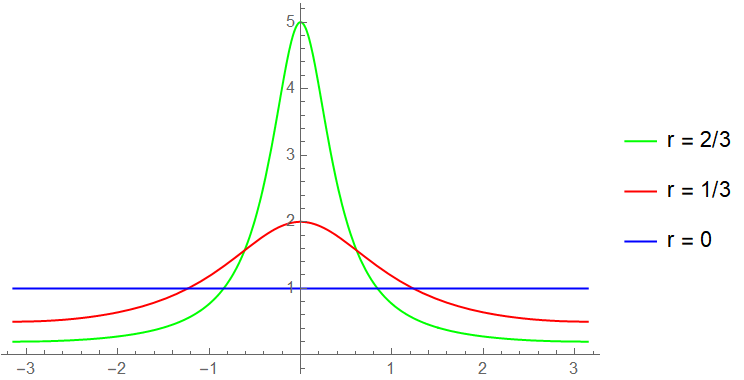
\includegraphics[width=\linewidth]{grafi.png}
        \caption{Graf Poissonovega jedra glede na vrednost spremenljivke $r$}
        \end{center}    
    \end{figure}

    Sedaj se vrnimo k reševanju Dirichletovega problema za enotski disk. 
    Spomnimo se, da smo za polinomske funkcije $h$ skonstruirali predpis razširitve, ki je rešila zastavljen problem. 
    Opazimo, da si sedaj lahko pomagamo z definiranim pojmom Poissonovega jedra in zapišemo:
    $$
    \widetilde{h}(r e^{i \theta}) = \int_{-\pi}^{\pi}{h(e^{i \varphi}) \bigg[\sum_{k = - \infty}^{\infty} r^{|k|} e^{- i k \varphi} e^{i k \theta}} \bigg]\frac{d \varphi}{2 \pi} = 
    \int_{-\pi}^{\pi}{h(e^{i \varphi}) P_r(\theta - \varphi)\frac{d \varphi}{2 \pi}}.
    $$
    Če (trigonometričen) polinom $h(e^{i\theta})$ (ki  bi seveda lahko zavzemal kompleksne vrednosti) zamenjamo s (trigonometričnim) polinomom $u(e^{i\theta})$, ki zavzema le realne vrednosti, se nam zgornja enakost v duhu 
    točke (7) trditve \ref{lastpk} še olepša. Takrat lahko namreč za $z = re^{i\theta} \in \mathbb{D}$ pišemo:
    \begin{equation}
        \label{realnidel}
        \begin{split}
            \widetilde{u}(z) = \widetilde{u}(r e^{i \theta}) = \int_{-\pi}^{\pi}{u(e^{i \varphi}) P_r(\theta - \varphi)\frac{d \varphi}{2 \pi}} = \int_{-\pi}^{\pi}{u(e^{i \varphi})~\text{Re}\bigg(\frac{1+re^{i(\theta - \varphi)}}{1-re^{i(\theta - \varphi)}}\bigg)\frac{d \varphi}{2 \pi}}= \\
            \int_{-\pi}^{\pi}{u(e^{i \varphi})~\text{Re}\bigg(\frac{e^{i\varphi}+re^{i\theta}}{e^{i\varphi}-re^{i\theta}}\bigg)\frac{d \varphi}{2 \pi}}=~\text{Re}~\bigg[\int_{-\pi}^{\pi}{u(e^{i \varphi})\bigg(\frac{e^{i\varphi}+z}{e^{i\varphi}-z}\bigg)\frac{d \varphi}{2 \pi}}\bigg].
        \end{split}
    \end{equation}
    S tem smo $\widetilde{u}(z)$ za $z \in \mathbb{D}$ izraziti kot realni del holomorfne funkcije, kar ne implicira le harmoničnost predpisa (po trditvi \ref{hh}), ampak tudi gladko odvisnost $\widetilde{u}(z)$ od spremenljivke $z$.
    \newline
    Posvetimo se sedaj spet iskanju splošne rešitve Dirichletovega problema. Zgoraj smo z intuitivno izpeljavo nevede že zapisali funkcijo, ki jo bomo sedaj vzeli za definicijo novega pojma. Pokazali smo, da to v splošnem pripelje do rešitve.

    \begin{definicija}
        \emph{Poissonov integral}, ki ga označimo z~$\widetilde{h}(z)$, zvezne funkcije $h(e^{i\theta})$, je funkcija, definirana na enotskem disku s predpisom
        $$
        \widetilde{h}(z) = \int_{-\pi}^{\pi}{h(e^{i\varphi}) P_r(\theta - \varphi)~\frac{d\varphi}{2 \pi}}~\text{, kjer je}~~z = r e^{i\theta} \in \mathbb{D}.
        $$
     \end{definicija}
     \begin{opomba}
        Ekvivalentno bi lahko definicijo Poissonovega integrala, zaradi 2 $\pi$ periodičnosti Poissonovega jedra, zapisali tudi kot:
        $$
        \widetilde{h}(z) = \int_{-\pi}^{\pi}{h\big(e^{i(\theta-\varphi)}\big) P_r(\varphi)~\frac{d\varphi}{2 \pi}}~\text{, kjer}~~z = r e^{i\theta} \in \mathbb{D}.
        $$
     \end{opomba}
     \begin{trditev}
        \label{lastpi}
        Za preslikavo $\Phi : h \mapsto \widetilde{h}$, t.j. preslikavo, ki zvezni funkciji $h$, definirani na $\partial \mathbb{D}$, priredi njen Poissonov integral, velja:
        \begin{enumerate}
            \item $\Phi$ je linearna preslikava, t.j. $\Phi(c_1 h_1 + c_2 h_2) = c_1 \widetilde{h_1} + c_2 \widetilde{h_2}$,
            \item $\Phi$ "ohranja omejenost", t.j. če je $|h| \leq M$ na $\partial \mathbb{D}$, potem je $|\widetilde{h}| \leq M$ na $\mathbb{D}$.
        \end{enumerate}
     \end{trditev}
     \begin{dokaz}
        $ $
        \begin{enumerate}
            \item Trditev trivialno sledi iz definicije Poissonovega integrala, zaradi linearnosti integrala. 
            \item Trditev sledi iz točke (2) in (3) trditve \ref{lastpk}.
        \end{enumerate}
     \end{dokaz}
        
     \begin{trditev}
        \label{obstoj}
        Naj bo $h$ zvezna kompleksna funkcija definirana na $\partial \mathbb{D}$. Rešitev Dirichletovega problema obstaja in je na $\mathbb{D}$ definirana kot Poissonov integral funkcije $h$.
        \newline
        Rečeno drugače, Poissonov integral zvezne kompleksne funkcije, definirane na $\partial \mathbb{D}$ je zvezna harmonična funkcija, definirana na $\mathbb{D}$, ki je zvezno harmonična razširitev $h$ na $\overline{\mathbb{D}}$, če jo dodefiniramo na $\mathbb{D}$.
     \end{trditev}
     \begin{dokaz}
        Trditev bomo dokazali v dveh korakih. Najprej dokažimo, da je Poissonov integral na $\mathbb{D}$ harmonična funkcija.
        Vemo, da lahko vsako kompleksno funkcijo $h$ razcepimo na njen realni in imaginarni del kot $h = u + iv$, pri čemer sta $u$ in $v$ funkciji, z zalogo vrednostjo znotraj realnih števil. 
        Zaradi linearnosti Poissonovega integrala, se lahko sedaj posebej skoncentriramo na Poissonov integral realnega dela (ki ga označimo z $\widetilde{u}$) in Poissonov integral imaginarnega dele (ki ga označimo z $\widetilde{v}$). 
        Tako, kot smo to naredili pri \ref{realnidel}, lahko vsakega izmed Poissonovih integralov $\widetilde{u}$ in $\widetilde{v}$ zapišemo kot realni del neke holomorfne funkcije, kar nam po trditvi \ref{hh} implicira harmoničnost $\widetilde{u}$ in $\widetilde{v}$.
        Zaradi opombe \ref{lin} nam to implicira tudi harmoničnost $\widetilde{h} = \widetilde{u} + i\widetilde{v}$ ter s tem dokaz prvega dela trditve. 
        \newline
        Za dokaz zveznosti na $\overline{\mathbb{D}}$ se moramo nekoliko bolj potruditi. Uporabili bomo lastnosti Poissonovega jedra iz trditve \ref{lastpk}. 
        Kot zvezna funkcija na kompaktu, je za $h$ na $\partial \mathbb{D}$ velja: 
        \begin{itemize}
            \item omejena, t.j.:$~\exists M: |h(e^{i\theta})| \leq M$ in 
            \item enakomerno zvezna, t.j.: $\forall \epsilon > 0, \exists \delta > 0: | \theta - \varphi | < \delta \Rightarrow |h(e^{i\theta}) - h(e^{i\varphi})| < \epsilon $.
        \end{itemize}
        Po točki (2) iz trditve \ref{lastpk} lahko zapišemo:
        $$
            \widetilde{h}(re^{i\theta}) - h(e^{i\theta}) = \int_{-\pi}^{\pi}{\bigg[h\big(e^{i(\theta - \varphi)}\big) - h(e^{i\theta})\bigg]P_r(\varphi)\frac{d\varphi}{2\pi}}.
        $$
        Sedaj vzamemo absolutno vrednost leve in desne strani enakosti, ter uporabimo trikotniško neenakost. Dobimo:
        $$
        |\widetilde{h}(re^{i\theta}) - h(e^{i\theta})| \leq \int_{-\pi}^{\pi}{\bigg| h\big(e^{i(\theta - \varphi)}\big) - h(e^{i\theta})\bigg|P_r(\varphi)\frac{d\varphi}{2\pi}}.
        $$
        Integral lahko razdelimo na dva dela, da bomo lahko uporabili enakomerno zveznost funkcije:
        $$
        |\widetilde{h}(re^{i\theta}) - h(e^{i\theta})| \leq \bigg(\int_{-\delta}^{\delta} + \int_{\delta \leq |\varphi| \le \pi}\bigg){\bigg| h\big(e^{i(\theta - \varphi)}\big) - h(e^{i\theta})\bigg|P_r(\varphi)\frac{d\varphi}{2\pi}}.
        $$
        Vrednosti znotraj prvega integral lahko zaradi enakomerne zveznosti navzgor ocenimo z $\epsilon$, vrednosti znotraj drugega integrala pa lahko prek omejenosti navzgor ocenimo kar z $2M$. 
        $$
        |\widetilde{h}(re^{i\theta}) - h(e^{i\theta})| \leq \epsilon \int_{-\delta}^{\delta}{P_r(\varphi) \frac{d\varphi}{2\pi}} + 2M\int_{\delta \leq |\varphi| \leq \pi}{P_r(\varphi)\frac{d\varphi}{2\pi}}.
        $$
        Vsakega od integralov lahko sedaj v duhu točke (2) trditve \ref{lastpk} navzgor ocenimo in dobimo:
        $$
        |\widetilde{h}(re^{i\theta}) - h(e^{i\theta})| \leq \epsilon  + 2M~\text{max}\{P_r(\varphi)~| ~\delta \leq |\varphi| \leq \pi \}.
        $$
        Sedaj uporabimo točko (6) trditve \ref{lastpk}, ki nam pove, da gre drugi sumand proti 0, ko gre $r$ proti 1. 
        Torej, za vsak $\widetilde{\epsilon} > 0$, pri $r$, ki je dovolj blizu 1, velja, da $|\widetilde{h}(re^{i\theta}) - h(e^{i\theta})| < \widetilde{\epsilon}$.
        Zveznost in s tem trditev je tako dokazana.
    \end{dokaz}
    \begin{posledica}
        Dirichletov problem za enotski disk je dobro postavljen matematičen problem. 
    \end{posledica}
    \begin{dokaz}
        Obstoj rešitve za vsako zvezno začetno podano funkcijo nam preko eksplicitne konstrukcije zagotavlja trditev \ref{obstoj}. 
        Enoličnost rešitve nam zagotavlja lema \ref{enolicno}, zvezna odvisnost rešitve od začetnih podatkov, pa je predpostavka problema (funkcija reši problem le v primeru, ko je zvezna na zaprtju enotskega diska, kar nam zagotavlja zvezno odvisnost od pogojev na robu diska oziroma zvezno odvisnost od začetnih pogojev).
    \end{dokaz}
    \begin{opomba}
        \label{alldisk}
        Dirichletov problem smo formulirali in reševali za enotski disk. Problem bi na podoben način lahko formulirali za poljubno območje $U$. 
        Kot začetni/robni pogoj bi podali zvezno funckijo $f$ (definirano na $\partial U$), ter iskali njeno razširitev $\widetilde{f}$ (na $\overline{U}$), tako da bi bila na $\overline{U}$ zvezna, 
        na $U$ harmonična, ter bi se zožitev $\widetilde{f}$ na $\partial U$ ujemala z $f$.
        V splošnem Dirichletovega problema znotraj diplomske naloge ne bomo reševali, vredno pa je omeniti, 
        da je bil prav enotski disk izbran zaradi preprostosti in bi lahko zgornji rezultat na podoben način zapisali za poljuben disk. To naredimo s pomočjo vpeljave novih spremenljivk ($z \mapsto az + b$) v Poissonov integral. 
        DOKONCAJ IZPELJAVO!
     \end{opomba}

     \begin{trditev}
        \label{ekvhlp}
        Naj bo $h$ zvezna funkcija, definirana na območju $U \subseteq \C$. Velja, da je $h$ harmonična funkcija natanko tedaj, ko ima lastnost povprečne vrednosti.
    \end{trditev}
    \begin{dokaz}
        Trditev \ref{harmonicnapovp} nam dokaže eno implikacijo. Dovolj je torej preveriti, da je zvezna funkcija $h$ z lastnostjo povprečne vrednosti na $U$ harmonična. 
        Dokaz temelji na že dokazanem obstoju rešitve Dirichletovega problema za enotski disk oziroma na opombi \ref{alldisk}, ki nam potrdi obstoj rešitve Dirichletovega problema za poljuben disk. 
        \newline
        Ker je $U$ območje za poljubno točko $z_0 \in U$ obstaja $r$, da je $\overline{\mathbb{D}}(z_0,r) \subseteq U$. Ker je $h$ zvezna na $U$, $h$ na $\partial \overline{\mathbb{D}}(z_0, r)$ določa robne/začetne pogoje za Dirichletov problem za disk $\mathbb{D}(z_0,r)$.
        Vemo, da rešitev $\widetilde{h}$ obstaja. 
        Kot harmonična funkcija na $\mathbb{D}(z_0, r)$ ima po trditvi \ref{harmonicnapovp} na $\mathbb{D}(z_0, r)$ lastnost povprečne vrednosti. 
        Oglejmo si sedaj funkcijo $g(z) = h(z) - \widetilde{h}(z)$ za $z \in \overline{\mathbb{D}}(z_0,r)$. 
        Kot razlika funkcij z lastnostjo povprečne vrednosti ima po trditvi \ref{linlpv} tudi $g$ na $\mathbb{D}(z_0, r)$ lastnost povprečne vrednosti in je kot razlika dveh zveznih funkcij zvezna na $\overline{D}(z_0, r)$.
        Vemo celo, da na $\partial \overline{\mathbb{D}}(z_0, r)$ velja $g \equiv 0$, saj je zožitev $\widetilde{h}$ na $\partial \overline{\mathbb{D}}(z_0,r)$ enaka $h$. 
        Po principu maksima, za funkcije z lastnostjo povprečne vrednosti je potem $g \equiv 0$. Oziroma $\widetilde{h} \equiv h$ na $\overline{\mathbb{D}}(z_0, r)$, kar nam da harmoničnost $h$ na $\mathbb{D}(z_0, r)$. 
        Dokazali smo torej, da je $h$ harmonična v okolici vsake točke $z_0$ v $U$. To pa nam že zagotavlja harmoničnost $h$ na $U$. 
    \end{dokaz}
    \begin{trditev}
        Naj bo $u$ zvezna funkcija z lastnostjo povprečne vrednosti, definirana na območju $D$. Potem je $u$ na $D$ gladka, $u \in C^{\infty}(D)$.
    \end{trditev}
    \begin{dokaz}
        Po trditvi \ref{ekvhlp} je $u$ harmonična, po trditvi \ref{gladkosth} pa zato tudi gladka.
    \end{dokaz}
\newpage
\section{Schwarzov princip zrcaljenja za harmonične funkcije}
    V tretjem poglavju, smo se že srečali s problemom razširitve podane funkcije do funkcije, ki mora zadoščati dodatnim pogojem. 
    Pri Dirichletovem problemu smo zahtevali harmoničnost razširitve na notranjosti območja/diska in zveznost razširitve na zaprtju območja/diska. 
    Pokazali smo, da to lahko naredimo s pomočjo Poissonovega integrala $\widetilde{h}$ kot:
    $$
        h^e(z) = 
        \begin{cases}
            h(z)~&z \in \partial \mathbb{D} \\
            \widetilde{h}(z)~&z \in \mathbb{D}
        \end{cases}.
    $$
    Problem, ki ga Schwarzov princip zrcaljenja reši je ne glede na drugačne začetne pogoje, iz vidika iskanja razširitve kljub temu blizu že rešenemu Dirichletovemu problemu.
    Glavna razlika je, da pri Schwarzovem principu zrcaljenja harmoničnost na območju vzamemo že za predpostavko, ter s pomočjo robnih zveznih začetnih pogojev poskušamo konstruirati harmonično razširitev na povsem novem območju podobne oblike.  
    Kot že nakazuje beseda zrcaljanje v imenu principa, bomo razširitev želeli konstruirati na "zrcalni sliki" prvotno definiranega območja. Prav zato bo potrebno predpostaviti nekaj simetrije.
    Spoznajmo sedaj nekaj osnovnih pojmov, ki nas bodo pripeljali do glavnega izreka.
    \begin{definicija}
        Naj bo $U$ območje. \emph{Zrcaljenje območja U čez realno os} definiramo kot $U^* = \{\overline{z}~|~z \in U\}$.
        \newline
        Pravimo, da je \emph{območje U simetrično glede na realno os}, če velja $U^* = U$.
        \newline
        Naj bo $u: U \to \mathbb{R}$. Potem lahko pri zgornjih oznakah definiramo $u^*: U^* \to \mathbb{R}$, kot $u^*(z) = u(\overline{z})$.
    \end{definicija}

    Naravno je pričakovati, da se zaradi dokaj preproste definicije $u^*$ lastnosti $u$ "prenesejo" tudi na $u^*$. 
    Spodnja lema nam to potrdi.

    \begin{lema}
        \label{lemaharm}
        Naj bo $U$ območje in $u: U \to \mathbb{R}$. Če je $u$ harmonična na $U$, je $u^*$ harmonična na $U^*$. 
    \end{lema}
    \begin{proof}
        Trditev lahko dokažemo na dva načina. Dokažimo najprej s pomočjo karakterizacije harmoničnih funkcij z lastnostjo povprečne vrednosti. 
        Ker je $u$ na $U$ harmonična ima na $U$ lastnost povprečne vrednosti.
        Sedaj je hitro jasno, da ima lastnost povprečne vrednosti tudi $u^*$ na $U^*$. 
        Iz trditve \ref{ekvhlp} potem sledi, da je $u^*$ na $U^*$ tudi harmonična.
        \newline
        Trditev je možno dokazati tudi kar direktno po definiciji, t.j. dokazati, da velja: $\frac{\partial^2 u^*}{\partial x^2} + \frac{\partial^2 u^*}{\partial y^2} = 0$. 
        Opazimo, da lahko $u^*$ (s pomočjo identifikacije $z = x + iy \leftrightarrow (x,y)$) zapišemo tudi kot kompozitum $u \circ ((x,y) \mapsto (x, -y))$. 
        Sedaj po definiciji parcialno odvajamo in dobimo enakosti:
        $$
            \frac{\partial u^*}{\partial y} = - \frac{\partial u }{\partial y},~~~~\frac{\partial^2 u^*}{\partial y^2} = \frac{\partial^2 u }{\partial y^2},~~~~\frac{\partial^2 u^*}{\partial x^2} = \frac{\partial^2 u }{\partial x^2},
        $$
        ki implicirajo:
        $$
            \frac{\partial^2 u^*}{\partial x^2} + \frac{\partial^2 u^*}{\partial y^2} = \frac{\partial^2 u}{\partial x^2} + \frac{\partial^2 u}{\partial y^2} = 0.
        $$
    \end{proof}
    \begin{lema}
        Če je $f$ holomorfna na območju $U$, je $g(z) = \overline{f({\overline{z}})}$ holomorfna na $U^*$.
    \end{lema}
    \begin{dokaz}
        Iz kompleksne analize vemo, da je dovolj pokazati, da tudi $g$ zadošča Cauchy-Riemannovemu sistemu enačb.
        \newline
        Pišimo: $f(z) = u(z) + iv(z)$ in $g(z) = p(z) + iq(z)$.
        Potem je $g(z) = u(\overline{z}) - iv(\overline{z})$ in zato $p(z) = u(\overline{z})~\text{ter}~q(z) = -v(\overline{z})$. 
        \newline
        Velja:
        \begin{equation*}
            \frac{\partial p}{\partial x} = \frac{\partial u}{\partial x} \overset{C-R}{=} \frac{\partial v}{\partial y} = - \bigg(- \frac{\partial q}{\partial y}\bigg) = \frac{\partial q}{\partial y}~~~\text{in}~~~
            \frac{\partial p}{\partial y} = -\frac{\partial u}{\partial y} \overset{C-R}{=} \frac{\partial v}{\partial x} = -\frac{\partial q}{\partial x}.
        \end{equation*}
        Alternativen dokaz si bralec lahko ogleda v REFERENCA.
    \end{dokaz}

    Sedaj smo pripravljeni na formulacijo in dokaz glavnega izreka.
    \begin{izrek}
        Naj bo $D \subseteq \C$ območje, simetrično glede na realno os. 
        Označimo $D^{+} = D \cap \{\text{Im} > 0\}$ in $D^{-} = D \cap \{\text{Im} < 0\}$.
        \newline
        Naj bo $u(z): D^{+} \to \mathbb{R}$ harmonična funkcija, za katero velja, da gre $u(z) \to 0$, ko gre $z \in D^{+}$ proti poljubni točki $D \cap \mathbb{R}$ t.j.: $$\lim_{\text{Im}(z) \to 0^+} u(z) = 0.$$
        Potem obstaja harmonična razširitev $u(z)$ na $D$, ki jo podaja predpis $u(\bar{z}) = - u(z)$ za $z \in D$:
        $$
            u^e(z) = 
            \begin{cases}
                u(z)~~&z \in D^{+}\\
                -u(\overline{z})~~&z \in D^{-}\\
                0~~ &z \in \mathbb{R}
            \end{cases}
            .
        $$
    \end{izrek}
    Preden se posvetimo dokazu, si na sliki oglejmo, kaj nam Schwarzov princip zrcaljenja zares omogoča.
    \begin{center}
        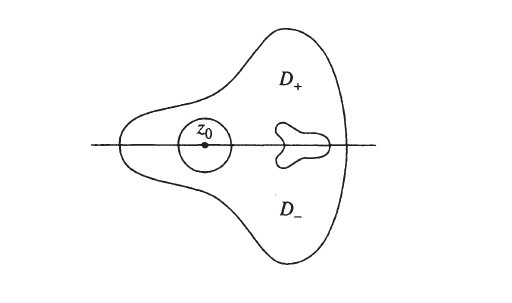
\includegraphics[width = 0.8 \textwidth]{schwarzov_princip_zrcaljenja.png}
    \end{center}
    Slika prikazuje glede na $\R$ simetrično območje $D \subseteq \C$. $D^{+}$ označuje območje, na katerem harmonično funkcijo $u$ poznamo, $D^{-}$ pa območje, na katerem lahko po izreku eksplicitno konstruiramo razširitev prek predpisa $u(\overline{z}) = - u(z)$.
    Vodoravna črta prikazuje odsek realne osi, na kateri bodo zaradi zahtevane zveznosti vrednosti trivialno poračunljive. 
    Točka $z_0$ in "majhen" disk okoli nje nakazujeta, da se bomo dokaza lotili z lastnostjo povprečne vrednosti.


    \begin{dokaz}
        Opazimo, da je $D$ disjunktna unija $D^+$, $D^-$ in $D^0 = D \cap \mathbb{R}$.
        Hitro je razvidno, da je $u^e$ na $D$ zaradi predpostavljene limite in ničelnih vrednosti na $D^0$ res zvezna. 
        \newline
        Posvetimo se dokazu harmoničnosti. Ker je $u^e$ na $D$ zvezna, je po trditvi \ref{ekvhlp} dovolj pokazati, da ima $u^e$ na $D$ lastnost povprečne vrednosti.
        Na $D^+$ je $u^e$ harmonična po predpostavki, na $D^-$ pa harmoničnost hitro preverimo prek leme \ref{lemaharm}. 
        Za poljubno točko $z_0 \in D^0$ pri dovolj majhnem $r$ (tako da je $\overline{\mathbb{D}}(z_0,r) \subseteq D$) velja, da se ob računanju povprečja paroma "zrcalne" vrednosti zaradi predpisa $u(\overline{z}) = - u(z)$ ravno odštejejo. 
        To pa že implicira, da je povprečje vrednosti na $\partial \overline{\mathbb{D}}(z_0,r)$ v poljubnem $z_0 \in D^0$ enaka $0$ in $u^e$ tudi v $z_0 \in D^0$ izpolnjuje lastnost povprečne vrednosti.
    \end{dokaz}

    HOLOMORFNE ?
\newpage

\bibliographystyle{siam}
\begin{thebibliography}{9}
    \bibitem{osnova}
    Theodore W. Gamelin \emph{Complex Analysis}, Springer (2001), Chapter X, str. 274 - 288

    \bibitem{mean value p}
    Weisstein, Eric W. \emph{Mean-Value Property}, v: From MathWorld--A Wolfram Web Resource, [ogled 22. 2. 2023], dostopno na \href{https://mathworld.wolfram.com/Mean-ValueProperty.html}{https://mathworld.wolfram.com/Mean-ValueProperty.html}
\end{thebibliography}

\end{document}